\documentclass[letter]{article}

\usepackage[margin=1in]{geometry} % make more efficient use of the page

\usepackage[utf8]{inputenc}

\usepackage{amsmath} % math tools
\usepackage{amsfonts} % math tools
\RequirePackage{amssymb} % math tools
\RequirePackage{amsbsy} % math tools

\renewcommand{\vec}[1]{\ensuremath{\boldsymbol{#1}}} % make vectors nicer

\usepackage{graphicx} % graphics
\usepackage{xcolor} % colored text

\usepackage{hyperref} % URLs and such
\usepackage{verbatim} % allows \verb-- command

\usepackage{algorithmicx} % algorithm environment
\usepackage{listings} % code listings

\usepackage{natbib} % bibliography

\newcommand{\mypath}[1]{\texttt{\path{#1}}}
\newcommand{\cmd}[1]{\begin{quote}\texttt{> #1}\end{quote}}


\title{CMDA 3634 \\ Lab 06 Report}
\author{Russell J. Hewett}
\date{}


\begin{document}

\maketitle

    \begin{enumerate}

        \item Include a screenshot of the welcome screen that you see when you log into Cascades. 
        \textbf{ANSWER:} % answer goes here

        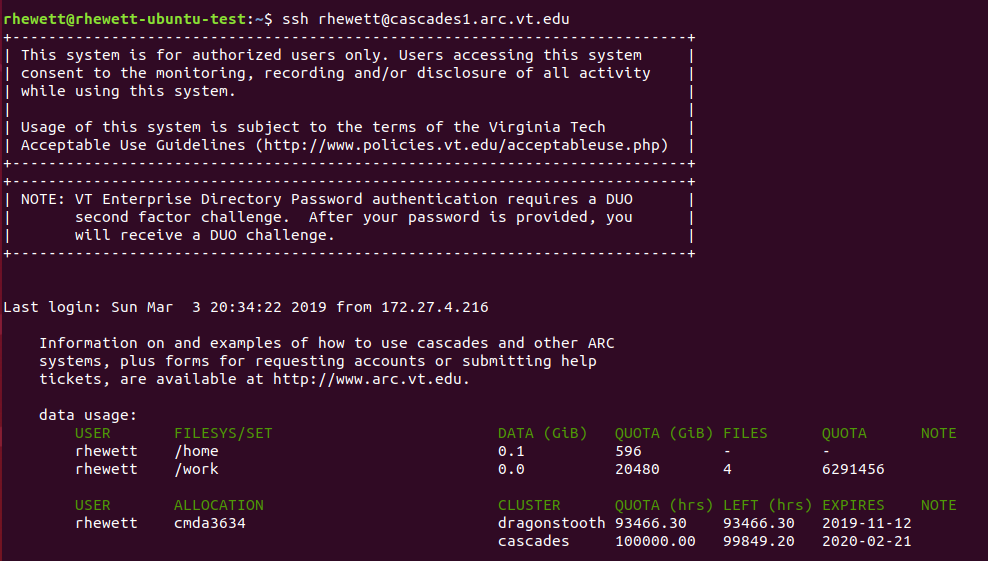
\includegraphics[scale=0.7]{login.png}

        \item Notice that the serial and parallel versions compute elapsed time in different ways.  Find a description of the \texttt{clock()} function online and think of something unexpected that it might return in our parallel version.
        \textbf{ANSWER:} % answer goes here

        Clock returns the number of ticks since the program is launched.  With OpenMP, it is not clear that clock will return the ticks from the master thread, or from a parallel thread, or even the sum over all threads.

        \item Explain in your own words why this algorithm works.  How many samples are necessary to approximate $\pi$ to 3 digits? 4 digits? 5 digits?  Create a plot which shows the quality of approximation as a function of the number of samples.
        \textbf{ANSWER:} % answer goes here

        This algorithm works because $\pi$ is proportional to the area of the circle.  The are of a unit radius circle is $\pi r^2 = \pi$ and the area of the section of the circle we used is therefor $\pi / 4.$  The area of the unit box is $r^2 = 1$, so dividing the samples in the circle section by the unit box gives an approximation to the area of the circle section.  When we multiply it by 4 we obtain an approximation of $\pi$.

        With approximately $10^8$ samples, $\pi$ to 5 digits: 3.141587.

        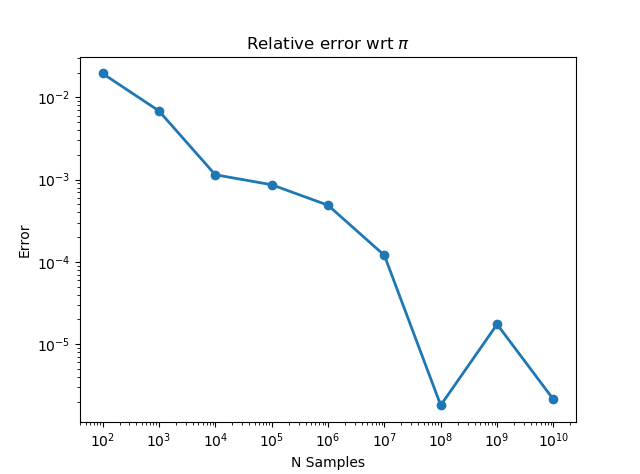
\includegraphics{convergence.png}


        \item Put your scaling plots for the laptop and Cascades in your pdf. 
        \textbf{ANSWER:} % answer goes here

        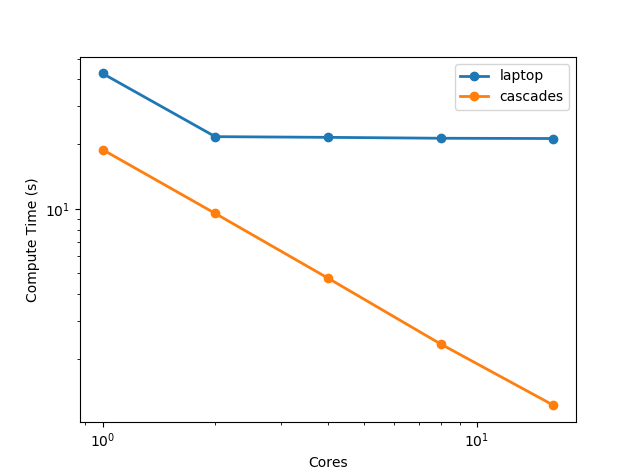
\includegraphics{timing.png}

        \item Observe that we plateau on the laptop (assuming you have less that 16 cores). Why is this?
        \textbf{ANSWER:} % answer goes here

        After 2 cores, the max allowed in my VM, the code executes sequentially (really with two threads only, concurrently), so we do not see any speedup after this point.

        \item The scaling for Cascades is approximately linear. Why is this? Can we expect this same scaling for other problems?
        \textbf{ANSWER:} % answer goes here

        We observe linear scaling on Cascades because the problem is embarassingly parallel (save for the reduction).  We do not expect this for problemsthat are not embarassingly parallel.

        \item Why is a \texttt{parallel for} on its own insufficient for completing \texttt{pi\_omp.c}?  List modifiers that we needed to add to the basic command.
        \textbf{ANSWER:} % answer goes here

        We cannot use a simple \texttt{parallel for} because it defaults all external variables to shared.  This would create an issue where all theads update the same random buffer, and compute on the same random buffer, negating the effect of random point selection.  To protect the buffer, it must be private.  Additionally, the counter must either be in a critical region or used in a reduction clause to ensure that we correctly obtain the total across all threads.  Because a critical region creates a sequential operation, the reduction clause is preferred.  Alternatively, we could implement the reduction ourselves, but it is best to let the compiler/run-time handle it.

        \item Other than the instructor or TAs, who did you receive assistance from on this assignment?
        \textbf{ANSWER:} % answer goes here
        
        No one.

    \end{enumerate}

\end{document}
